%% LyX 1.1 created this file.  For more info, see http://www.lyx.org/.
%% Do not edit unless you really know what you are doing.
\documentclass[10pt,oneside,british]{book}
\usepackage{times}
\usepackage[T1]{fontenc}
\usepackage[latin1]{inputenc}
\usepackage{a4wide}
\usepackage{fancyhdr}
\pagestyle{fancy}
\usepackage{babel}
\setcounter{secnumdepth}{3}
\setcounter{tocdepth}{3}
\setlength\parskip{\smallskipamount}
\setlength\parindent{0pt}
\usepackage{graphics}

\makeatletter

%%%%%%%%%%%%%%%%%%%%%%%%%%%%%% LyX specific LaTeX commands.
\providecommand{\LyX}{L\kern-.1667em\lower.25em\hbox{Y}\kern-.125emX\@}
\newenvironment{LyXParagraphIndent}[1]%
{
  \begin{list}{}{%
    \setlength\topsep{0pt}%
    \addtolength{\leftmargin}{#1}
    \setlength\parsep{0pt plus 1pt}%
  }
  \item[]
}
{\end{list}}

%%%%%%%%%%%%%%%%%%%%%%%%%%%%%% User specified LaTeX commands.
\renewcommand{\headrulewidth}{0.4pt}
\renewcommand{\footrulewidth}{0.4pt}
\lhead{\resizebox{1in}{!}{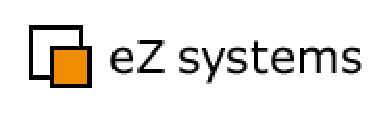
\includegraphics{icons/ezsystems.eps}}}
\rhead{}
\chead{}

\makeatother
\begin{document}

\title{eZ publish Installation Guide}


\author{\resizebox*{0.75\columnwidth}{!}{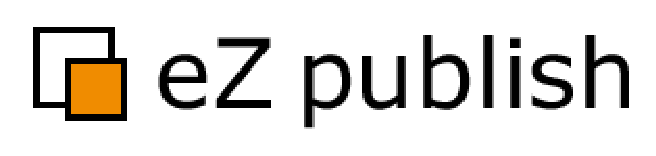
\includegraphics{icons/ezpublish.eps}} }

\maketitle
\resizebox*{!}{0.2in}{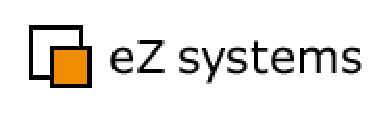
\includegraphics{icons/ezsystems.eps}} The
double squares and eZ are trademarks belonging to eZ systems of Norway,
registration number NO 981 601 564 (http://www.brreg.no/oppslag/enhet/detalj.ssc?orgnr=981601564).

All images and text herein is Copyright 2001 eZ systems.

eZ publish is a software package released under the GPL lisence (http://www.gnu.org/copyleft/gpl.html),
its primary point of distribution and information is http://devel.ez.no/

\tableofcontents{}


\chapter{Introduction\label{chptr: introduction}}

\begin{quote}
\textbf{{}``He who asks is a fool for five minutes, but he who does
not ask remains a fool forever.{}''} - \-
\end{quote}
eZ publish is a content management system, among a lot of other things.
This installation manual will try to cover the job of installing eZ
publish on your server.

This manual covers installation on a Red Hat Linux system; most of
what is described here can also be applied to other installations,
especially if your system uses RPM for installation. For other systems
you would need to do a lot of compiling yourself to make this work,
or apply the system's own package manager.

Finding packages can be done dirctly from vendor sites, though you
might not be guaranteed that you'll find the package you need. In
such instances you need to download the source directly from the software
developer.

Different distribution sites for different Unix systems are:

\begin{itemize}
\item AIX http://www-frec.bull.com/docs/download.htm
\item Debian http://www.debian.org/distrib/ftplist
\item IRIX http://freeware.sgi.com/
\item HP-UX http://hpux.connect.org.uk/
\item Red Hat Linux http://www.redhat.com/apps/download and http://rpmfind.net.
\item SCOOpen Server/Unixware http://www.sco.com/skunkware/
\item SuSE Linux http://www.suse.com/us/support/download/index.html
\item Sun http://www.sunfreeware.com/
\end{itemize}
You can also try {}``The Written Word{}'' {\footnotesize (ftp://ftp.thewrittenword.com/packages/free/by-name/gcc-2.95.2/)}
for binaries for Solaris 2.5.1, 2.6, 2.7/SPARC, 2.7/Intel, IRIX 6.2,
6.5, Digital UNIX 4.0D, HP-UX 10.20, and HP-UX.

The addresses to the software developers will be given where apropriate
in the text.

A line starting with a hash-sign {}``\#{}'' are input from the user
to the shell.


\section{Pre-Configured Hosting}

It is possible to get pre-configured hosting services where you can
install and manage your eZ publish site with ease. Read more about
our hosting partners at eZ systems web site {\footnotesize (http://en.ez.no/article/articlestatic/73)}.


\section{Pre-Configured Hardware}

It is possible to order pre-configured hardware from eZ systems. You
can order through or web shop {\footnotesize (http://sourceprovider.com/)}.


\chapter{Pre-requisites\label{chptr: pre-requisites}}


\section{Needed Privileges}

For the standard installation (and for the moment the only method)
of eZ publish you will need to have the following privileges on your
system:

\begin{itemize}
\item Access to Apache's httpd.conf
\item \footnote{%
You will have to install the gcc compiler on your system, see chapter
\ref{chptr: introduction} for a list of sites providing software
for different Unixes.
}Access to compiler
\item \footnote{%
You must run certain scripts during installation. Some of them are
just creating links to different directories; you might therefore
just create those links via FTP.
}Access to a shell
\item \footnote{%
Only needed if you want to use the eZ news feed module for regular
updates of headlines imported from other sites.
}Access to cron jobs
\item Access to Apache's modules
\item Access to a MySQL database
\item You might also need the privilege to add new libraries to your system.
\end{itemize}
You might also use other web servers than apache, but then you're
on your own since we haven't tested eZ publish on other configurations.
If you do try another web server, please keep a log of what you do
and submit it to us (pkej@ez.no) for inclusion in future versions
of this manual.


\section{Needed Software}

You also need to download and install the following packages, if they
aren't present on your system already:

\begin{itemize}
\item \footnote{%
eZ publish requires MySQL for storage of its data.
}MySQL (http://www.mysql.com) version 3.23 or later.
\item \footnote{%
Needed by eZ article. If you wish to use the default article renderer
you need libXml2 installed. You can create your own renderers if you
don't want to use the default.
}libXml2 (http://xmlsoft.org/\#Downloads) version 2.2.7 or later.
\item \footnote{%
Needed by eZ news feeds parsers. If you wish to include headlines
from external sites (example developer.ez.no or slashdot.org) then
you need this installed. You can create your own parsers if you don't
want to use the default.
}libQdom (http://www.trolltech.com) is a part of QT, you need version
2.2.3 or later.
\item \footnote{%
Needed by eZ article, eZ image catalogue, and all modules using images.
You need only the command line version.
}ImageMagick (http://www.imagemagick.org/) newest version
\item \footnote{%
It is always recommended to run the latest Apache release, though
eZ publish shouldn't be very picky with the Apache versions. We've
used eZ publish with Apache 1.3.13, some have reported that Apache
1.3.9 isn't useful.
}Apache (http://httpd.apache.org/) latest 1.3 release.
\item Any and all modules you need for apache in addition to mod\_php. (http://modules.apache.org/)
\item \footnote{%
eZ publish uses references for objects and foreach loops. Only version
4.0.4pl1 and later supports both of these features satisfactorily.
}PHP (http://www.php.net/) version 4.0.4pl1 or later, you need the
source code version.
\item eZ publish (http://developer.ez.no/) verision 2.0 or later stable
releases.
\end{itemize}
The libraries and php will appear pre-compiled for Linux i386 on http://developer.ez.no
in the future. The software is listed in the order of installation.


\section{Which Software is Already Installed?}


\subsection{Systems Using RPM}

RPM is a system for distributing pre-compiled software. The packages
also contain pre-configured settings and initialisation files, leaving
almost nothing to the user, except deciding what to install.

To check if a package is available on your system you can run the
following command (RPM based systems {}``rpm -qa | grep <name of
program/library>{}''. If you need to know where you can find the
different files from that package you can follow up on the previous
command with the following {}``rpm -ql <rpm name>{}''. RPM name
is one of the returned names from the previous command, example: 

\begin{LyXParagraphIndent}{5mm}
\medskip{}
\texttt{\# pkej@vogol:/etc/httpd > rpm -qa | grep libxml}

\texttt{libxml-1.8.7-80}

\texttt{libxmld-1.8.7-80}

\texttt{\# pkej@vogol:/etc/httpd > rpm -ql libxml-1.8.7-80}

\texttt{/usr/bin/xml-config}

\texttt{/usr/lib/libxml.so.1}

\texttt{/usr/lib/libxml.so.1.8.7}

\texttt{/usr/share/doc/packages/libxml}

\texttt{/usr/share/doc/packages/libxml/AUTHORS}

\texttt{/usr/share/doc/packages/libxml/COPYING}

\texttt{/usr/share/doc/packages/libxml/COPYING.LIB}

\texttt{/usr/share/doc/packages/libxml/NEWS}

\texttt{/usr/share/doc/packages/libxml/README}

\texttt{/usr/share/doc/packages/libxml/TODO}

\end{LyXParagraphIndent}

You should test for qt, libxml and imagemagik to check if those are
installed and working.


\subsection{IRIX}

By accessing the software manager (you must be root) you can get a
list of installed software, scroll or search that list to find the
packages you're interested in. Double click on the tabs to the left
to get information about where specific files are installed.


\subsection{Other Systems}

On other systems you should read the documentation for that system
to learn how to find out what software is already installed.

You could try to use the command {}``find{}'' to find the software.
It is used thus: {}``find . -name \textbackslash{}{*}<program name>\textbackslash{}{*}{}''
from the /usr/, /local/ , /lib/, /share/ directories. In extreme cases
you could try from the root of the system, but this will take a long
time and will also hog resources on your computer. Therefore we urge
you to learn how to use the proper installation features of your system
to find the software already installed.


\section{Installation of Required Software}

If you've found pre-compiled versions of all the software packaged
for use with an installation tool, you just have to install that software
using the tool. Instructioins for its usage is often found using the
command {}``man <installation tool name>{}'' or by reading your
system's documentation or the supplier's website.

If you've had to download source code you will find instructions on
how to compile and install the software you've downloaded at the software
developer's website. This requires a bit of knowledge and you should
only undertake this if you feel confident about the job.

This manual will only cover configuration of the software needed and
compilation of PHP to use the other software.


\subsection{Important Notice}

You should read all the README, INSTALL and similar files found with
the software packages you download. They often contain tips on how
to configure, compile and install the software on your system. It
will save you a lot of time and aggravation if you follow instructions
supplied with the software.

If problems arise during installation of the software, please turn
to the suppliers support forums, mailing list archives and FAQs, your
questions will often be answered there. If the supplier's forums doesn't
seem to help you, you should check the support forums at our site.

You should always do a search of the forums before posting any questions.


\chapter{Compile Configuration}


\section{PHP}


\subsection{Unpacking}

After you have downloaded PHP you need to unpack it somewhere where
you can compile and configure the software. To unpack run the command:

\begin{itemize}
\item \texttt{\# tar zxvf php-4.0.x.tar.gz}
\end{itemize}
Where the x is the version of php you've downloaded. Then you need
to move into the directory you extracted php into:

\begin{itemize}
\item \texttt{\# cd php-4.0.x}
\end{itemize}

\subsection{Configuration}

You'll need either an apache module or a command line version of PHP
to use eZ publish on your website. We recommend you use PHP as an
apache module. You will also need the command line version if you
want to use the cron jobs for periodical updates of the eZ news feed
module.

Thus for our recommended installation of PHP you need both the command
line and module versions of PHP.


\subsubsection{Common}

Both the command line and apache module versions need to have the
following configurations added to the configuration tool:

\begin{description}
\item [--enable-trans-sid]This lets PHP use session id's which don't rely
on cookies. It does not disable normal cookie based sessions.\\
({\footnotesize http://www.php.net/manual/en/install.configure.php\#install.configure.enable-trans-sid})
\item [--with-mysql]This tells PHP that the mysql functionality should be
used.\\
({\footnotesize http://www.php.net/manual/en/install.configure.php\#install.configure.with-mysql})
\item [--enable-magic-quotes]This tells PHP to enable magic quotes by default.
you can also turn this feature on and off on a directory by directory
basis in either the {}``.htaccess{}'' files (if you use them) or
in the setup of the virtual server in {}``httpd.conf{}''.\\
({\footnotesize http://www.php.net/manual/en/install.configure.php\#install.configure.enable-magic-quotes})
\item [--with-dom]This configures PHP to include libxml. {\footnotesize }\\
{\footnotesize (http://www.php.net/manual/en/install.configure.php\#install.configure.with-dom)}{\footnotesize \par}
\item [--with-qtdom]This configures PHP to include libqdom. It isn't up
on the PHP site with a link, but it works as --with-dom.
\end{description}
You should also go through the web page: {\footnotesize http://www.php.net/manual/en/install.configure.php}
and make sure that there isn't other functionality you would like
to have included.


\subsubsection{Command Line}

The default is to create a command line version of PHP. Therefore
you don't need to add more configuration options for this.


\subsubsection{Apache Module}

To build an apache module you need to add:

\begin{description}
\item [--with-apxs]This compiles PHP as an apache module. {\footnotesize }\\
{\footnotesize (http://www.php.net/manual/en/install.configure.php\#install.configure.with-apxs)}{\footnotesize \par}
\end{description}

\subsubsection{Other Web Servers}

We haven't tested our software with other web servers than apache.
If you need to try out other web servers, read this document {\footnotesize http://www.php.net/manual/en/install.configure.php\#install.configure.servers}
to learn how you configure for the web server you will be using.


\subsubsection{Creating the Configuration}

Now you just have to run the {}``./configure{}'' program with the
apropriate configuration directives which we discussed in the preceeding
sections, for an apache module you'd do the following:

\begin{itemize}
\item \texttt{\# ./configure -{}-enable-trans-sid -{}-with-mysql -{}-with-magic-quotes
-{}-with-apxs -{}-with-dom -{}-with-qtdom}
\end{itemize}
Remember that to compile a script/cgi version you'd need to change
that line to:

\begin{itemize}
\item \texttt{\# ./configure -{}-enable-trans-sid -{}-with-mysql -{}-with-magic-quotes
-{}-with-dom -{}-with-qtdom}
\end{itemize}

\subsection{Compilation}

To compile you need to run the command {}``make{}'':

\begin{itemize}
\item \texttt{make}
\end{itemize}

\subsection{Installation}

To install your new PHP package you need to run the following command:

\begin{itemize}
\item \texttt{make install}
\end{itemize}

\chapter{Apache Configuration}

For the moment we have only one solution for configuring apache. There
are other methods, and we'll document them in the future.


\section{Dual Virtual Host}

This set up is based on having two different virtual hosts for your
administration back-end and the main site. The main site would typically
be known as {}``www.yoursite.com{}'' and the administration would
be {}``admin.yoursite.com{}''; the names are up to you, theoretically
you could have different names, for example {}``mysite.yoursite.com{}''
and {}``administration.mysite.com{}''.

The virtual host is configured through the {}``httpd.conf{}'' file
which is the main configuration of Apache. Following is an example
of such a host, remember to exchange everything within brackets ({}``{[}{}``
and {}``{]}{}'') with your preferred and local settings and also
remove the brackets.

\begin{LyXParagraphIndent}{2mm}
\texttt{\scriptsize \# User site }{\scriptsize \par}

\texttt{\scriptsize <VirtualHost yourdomain.org> }{\scriptsize \par}

\texttt{\scriptsize <Directory {[}/your/apache/documentroot/{]}> }{\scriptsize \par}

\texttt{\scriptsize Options FollowSymLinks Indexes ExecCGI }{\scriptsize \par}

\texttt{\scriptsize AllowOverride None }{\scriptsize \par}

\texttt{\scriptsize </Directory>}{\scriptsize \par}

\texttt{\scriptsize RewriteEngine On}{\scriptsize \par}

\footnote{%
This line and the next should be written on the same line in your
apache.conf file.
}\texttt{\scriptsize RewriteRule \textasciicircum{}/filemanager/filedownload/({[}\textasciicircum{}/{]}+)/(.{*})\$
}~\\
\texttt{\scriptsize {[}/your/apache/documentroot{]}/publish\_dist/ezfilemanager/files/\$1
{[}T=\char`\"{}application/oct-stream\char`\"{},S=1{]}}{\scriptsize \par}

\texttt{\scriptsize RewriteRule !\textbackslash{}.(gif|css|jpg|png)\$
{[}/your/apache/documentroot{]}/index.php}{\scriptsize \par}

\texttt{\scriptsize ServerAdmin {[}your\_mail@domain.no{]}}{\scriptsize \par}

\texttt{\scriptsize DocumentRoot {[}/your/apache/documentroot/{]}}{\scriptsize \par}

\texttt{\scriptsize ServerName {[}yourdomain.org{]}}{\scriptsize \par}

\texttt{\scriptsize ServerAlias {[}www.yourdomain.org{]}}{\scriptsize \par}

\texttt{\scriptsize </VirtualHost>}{\scriptsize \par}

\texttt{\scriptsize \# Admin site }{\scriptsize \par}

\texttt{\scriptsize <VirtualHost admin.yourdomain.org> }{\scriptsize \par}

\texttt{\scriptsize <Directory {[}/your/apache/documentroot{]}/admin> }{\scriptsize \par}

\texttt{\scriptsize Options FollowSymLinks Indexes ExecCGI }{\scriptsize \par}

\texttt{\scriptsize AllowOverride None }{\scriptsize \par}

\texttt{\scriptsize </Directory> }{\scriptsize \par}

\texttt{\scriptsize RewriteEngine On }{\scriptsize \par}

\texttt{\scriptsize RewriteRule !\textbackslash{}.(gif|css|jpg|png)\$
{[}/your/apache/documentroot{]}/admin/index.php}{\scriptsize \par}

\texttt{\scriptsize ServerAdmin {[}your\_mail@domain.no{]}}{\scriptsize \par}

\texttt{\scriptsize DocumentRoot {[}/your/apache/documentroot/{]}admin}{\scriptsize \par}

\texttt{\scriptsize ServerName {[}admin.yourdomain.org{]}}{\scriptsize \par}

\texttt{\scriptsize ServerAlias {[}admin.yourdomain.org{]}}{\scriptsize \par}

\texttt{\scriptsize </VirtualHost>}{\scriptsize \par}

\end{LyXParagraphIndent}

The format of the {}``httpd.conf{}'' file is covered at http://httpd.apache.org/docs/
for a complete understanding of the above information you'll need
to read that documentation. You should note that you can't use any
rewrite ruels inside the <directory> part within the <VirtualHost>.

If you didn't compile PHP with magic quotes; or other software relies
on PHP not using magic quotes you can add the following line into
each virtual host section:

\begin{itemize}
\item \texttt{php\_value magic\_quotes\_gpc 1}
\end{itemize}

\chapter{eZ publish Installation}


\section{Database}

Now you need to create a database in MySQL, the default name we use
is publish, but you can change that to whatever pleases you.

\begin{itemize}
\item \texttt{\# mysqladmin create publish}
\end{itemize}
Add a publish user in MySQL. To add a user you can use the MySQL client
to log on to mysql and then create the user:

\begin{itemize}
\item \texttt{\# mysql>grant all on publish.{*} to publish@localhost identified
by \char`\"{}secret\char`\"{};}
\end{itemize}
where secret is your password. Then you need to add the default eZ
publish data into your newly created database: 

\begin{itemize}
\item \texttt{\# mysql -uroot -p publish < sql/publish.sql}
\end{itemize}

\section{Program Files}

The next step is to install the eZ publish package in your document
root directory. First you need to unpack the software in a temporary
directory:

\begin{itemize}
\item \texttt{\# cd /tmp}
\item \texttt{\# tar zxvf /path/to/ezpublish-2.0.tar.gz}
\end{itemize}
The next step is to move the files to your document root:

\begin{itemize}
\item \texttt{\# mv /tmp/publish\_dist /your/apache/documentroot}
\end{itemize}
When all this is done you need to tell eZ publish a little about the
site you're running. You'll need to edit the {}``site.ini{}'' file
which you will find in the document root:

\begin{itemize}
\item \texttt{\# cd /your/apache/documentroot}
\item \texttt{\# vi site.ini}
\end{itemize}
Instead of vi you can use your preferred text editor. You'll need
to add information about the username, hostname and password of your
database. More information on what you can do with {}``site.ini{}''
can be found in the {}``eZ publish Customisation Guide{}''.

The next important step is to run the script modfix. This script will
create symbolic links needed and set permissions.

\begin{itemize}
\item \texttt{\# ./modfix.sh}
\end{itemize}

\chapter{Now What?}

After installing eZ publish you can test your site through the URL
http://www.yoursite.com/ and you can administrate your site from the
URL http://admin.yoursite.com/, of course, if you did anything different
the names of the admin and the public site might be different.

\emph{NOTE:} The default user name and password for your site will
be admin/publish. Remember to change the password.

The next manual you should read is the {}``eZ publish Customisation
Guide{}'', it tells you how to configure the software to use the
functionality you want, as well as how you change the templates to
suit your needs.

When you're finished with the design and the initial testing you can
head over to http://zez.org/ for articles about community building
as well as programming, or you can visit http://developer.ez.no for
updates, articles about eZ publish and how to work with it, as well
as keeping abreast of new developments.


\chapter{Trouble Shooting}


\section{Problems During Installation}


\subsection{FreeBSD 4.2 and libxml2}

The current version (2.2.11) installs itself as /usr/local/lib/libxml2.a|so
and goes unrecognized by configure (PHP). Link the fiels to /usr/local/lib/libxml.a|so.


\subsection{Missing Compiler/Can not Compile (C++/C)}

The ImageMagick package requires the GCC compiler. You'll need to
download that compiler and install it on your system. In the introduction
(see chapter \ref{chptr: introduction}) I listed some sites where
you can download pre-compiled versions of software for some different
Unix versions.

If you can't find a pre-compiled version try the GCC Home Page (http://gcc.gnu.org/).


\section{Problems After Installation}


\subsection{Permission Denied}

\texttt{\small Warning: fopen(\char`\"{}site.ini\char`\"{},\char`\"{}r+\char`\"{})}{\small \par}

\texttt{\small Permission denied in classes/INIFile.php on line 80}{\small \par}

If you get this error message you need to run the modfix.sh script.
\end{document}
